% $Header: https://svn.ita.chalmers.se/repos/security/edu/course/computer_security/trunk/assignment/3/template/latex/report.tex 611 2013-02-20 13:33:23Z pk@CHALMERS.SE $
%
%

\documentclass[a4paper,twoside,11pt]{article}

\usepackage{etoolbox}
\usepackage[utf8]{inputenc}
\usepackage{microtype}

\usepackage[pdftex,hidelinks]{hyperref}
\hypersetup{
    pdfstartview=FitH,
%    pdftitle={},
%    pdfauthor={},
%    pdfsubject={},
%    pdfkeywords={}
%    bookmarks,
%    bookmarksopen,
%    colorlinks,
%    linkcolor=blue,
%    citecolor=blue,
%    urlcolor=black,
}
\usepackage[english]{babel}
\usepackage[T1]{fontenc}
\usepackage{geometry}
\usepackage{fancyhdr}


% Setup bibliography
\usepackage{csquotes}
\usepackage[backend=biber, natbib=true, maxnames=2, minnames=1, 
maxbibnames=10, minbibnames=6, citestyle=numeric-comp, sorting=none, 
firstinits=true]{biblatex}
%\providecommand{\bibfont}{\footnotesize}
%\renewcommand{\bibfont}{\footnotesize}

% To be used for colors
\usepackage{color}
\usepackage[usenames,dvipsnames,svgnames,table]{xcolor}

% Useful Packages
\usepackage{amsmath}
\usepackage{amsthm}
\usepackage{amsfonts}

\usepackage{graphicx}
\usepackage{breakurl}

% Nice tables
\usepackage{hhline}
\usepackage{booktabs}
\usepackage{caption}

\usepackage{pdfpages}
\def\arraystretch{1.3}
% Loading ToDo notes
\usepackage{setspace}
\usepackage{todonotes}
\usepackage{titlesec}
\newcommand{\inlinetodo}[2][]{\todo[caption={#2},inline,#1]{#2}}
\newcommand{\checknote}[2][]{\todo[caption={#2},size=\small,color=yellow!40,#1]{\begin{spacing}{0.5}#2\end{spacing}}}


\makeatletter
\renewcommand{\title}[1]{\gdef\@title{#1}}
\renewcommand{\author}[1]{\gdef\@author{#1}}
\renewcommand{\date}[1]{\gdef\@date{#1}}
\newcommand{\report}[1]{\gdef\@report{#1}}
\newcommand{\group}[1]{\gdef\@group{#1}}
\newcommand{\version}[1]{\gdef\@version{#1}}

\newcommand{\maketitlepage}{%
 \thispagestyle{empty}
 {
  \vspace{2cm}
  {\huge\centering\@title\par}
  \vspace{2cm}
  {\centering\@report\par}
  \vspace{2cm}
  {\centering\@author\par}
  \vskip1em
  {\centering\small Group~\@group\par}
  \vfill
  {\centering Version no:~\@version
   \vskip1em
   \@date\par}
  \vspace{2cm}

  \newpage
  \thispagestyle{empty}
  \mbox{}
 }
}
\makeatother

\renewcommand{\maketitle}{%
 \pagestyle{plain}
 \setcounter{page}{-100}
 \maketitlepage
 \newpage
 \pagenumbering{roman}
 \tableofcontents
 \listoftables
 \listoffigures


 \cleardoublepage
 \pagenumbering{arabic}
}

% Title and Authors. This should be updated by you!
\title{Vulnerability Scanning with OpenVAS}
\report{Laboratory Report in EDA263/DAT641 Computer Security}
\author{Oskar Åkergren\\Pär Svedberg}
\group{1}
\date{\today}
\version{1.1}

% The bilbiography to include
\addbibresource{report.bib}


\begin{document}

\maketitle % Make titlepage

\newcommand{\sectionbreak}{\clearpage}

\section{Introduction} \label{sec:intro}

\inlinetodo{This section shall introduce the reader to the subject addressed by the report. It should include a description of the purpose of the report, i.e., a formulation of the problem to which the report provides an answer. Try to motivate the reader to keep reading your report to know more about vulnerability scanning and OpenVAS. 
\newline
~\ \newline
The last paragraph should consist of a ''roadmap'' of the report, e.g., The 
rest of the paper is organized as follows: Section~\ref{sec:setup} 
provides\ldots\nocite{*}}

\textbf{\newline
~\ \newline
General Notes about the report:
\newline
}

\inlinetodo{The report should be self-contained and descriptive. It is not allowed to use the lab-pm as a reference. You may read and use information from lap-pm, but do not copy text from any reference.
\newline
~\ \newline
\inlinetodo{The purpose of the report is to train your skills in technical writing. So try to make it well-written and well-structured. In each section, it is not enough to only present the results. Try to be descriptive, do some research and elaborate on the results.}}


\inlinetodo{If you need information on \LaTeX, \citep{latex-wikibook} is a 
good place to start\ldots}
\section{Description of OpenVAS Setup} \label{sec:setup}

Open Vulnerability Assessment System is a system that collects multiple services and tools, called “Network Vulnerability Tests” (NVT) and presents them in a single interface, allowing the user to combine them to a thoroughly vulnerability scan \cite{openvas}. \\

\noindent The logical layout of the network scanned for this report is presented in Figure \ref{fig:setup}, where the target is “rome.secnet”. OpenVAS is installed on the intermediate server between the target and our client machine. \\

\noindent Scanning a host is a method to control in which ways a system is open to the outside, and it is one of the methods an attacker might conduct to search for entry points in a system \cite{wiki}. There are several types of vulnerability scans, such as “port scan”, “database scan”, “web application security scan” and others \cite{hk}. \\

\noindent The scans used in this report is in order: “port scan”, “service fingerprinting” and “network vulnerability scan”. The different scans will produce a list of open ports found on the host, combined with a fingerprint scan that will search through these open ports and generate a fingerprint of what type of services that are behind these ports. The fingerprint will contain the available information, such as the names and versions of services. \\

\noindent In the scans we expect a result in the form of information about open ports and the services behind them, marked with the security risk of each port and/or service.\\

\noindent To perform a scan with OpenVAS, the system needs to be installed on a server. In the interface of OpenVAS, the user choose which types of NVTs should be conducted with each scan, what port range to use and which target in the network the scan is aimed at. \\

\noindent To detect as many open ports as possible within a reasonable time, the optimized OpenVAS default port range was chosen. This setting checks a 
wide range of well known ports, and is optimized to lower the time 
consumption of the scan, compared to a scan over all ports.\\

%\noindent The aim of this report is to detect as many open ports as possible, within reason. The host is not known to have any extraordinary security issues, so the OpenVAS default port range was chosen as a suitable range, as it provides a wide range of well known ports.



\begin{figure}[hbt]
  \centering
  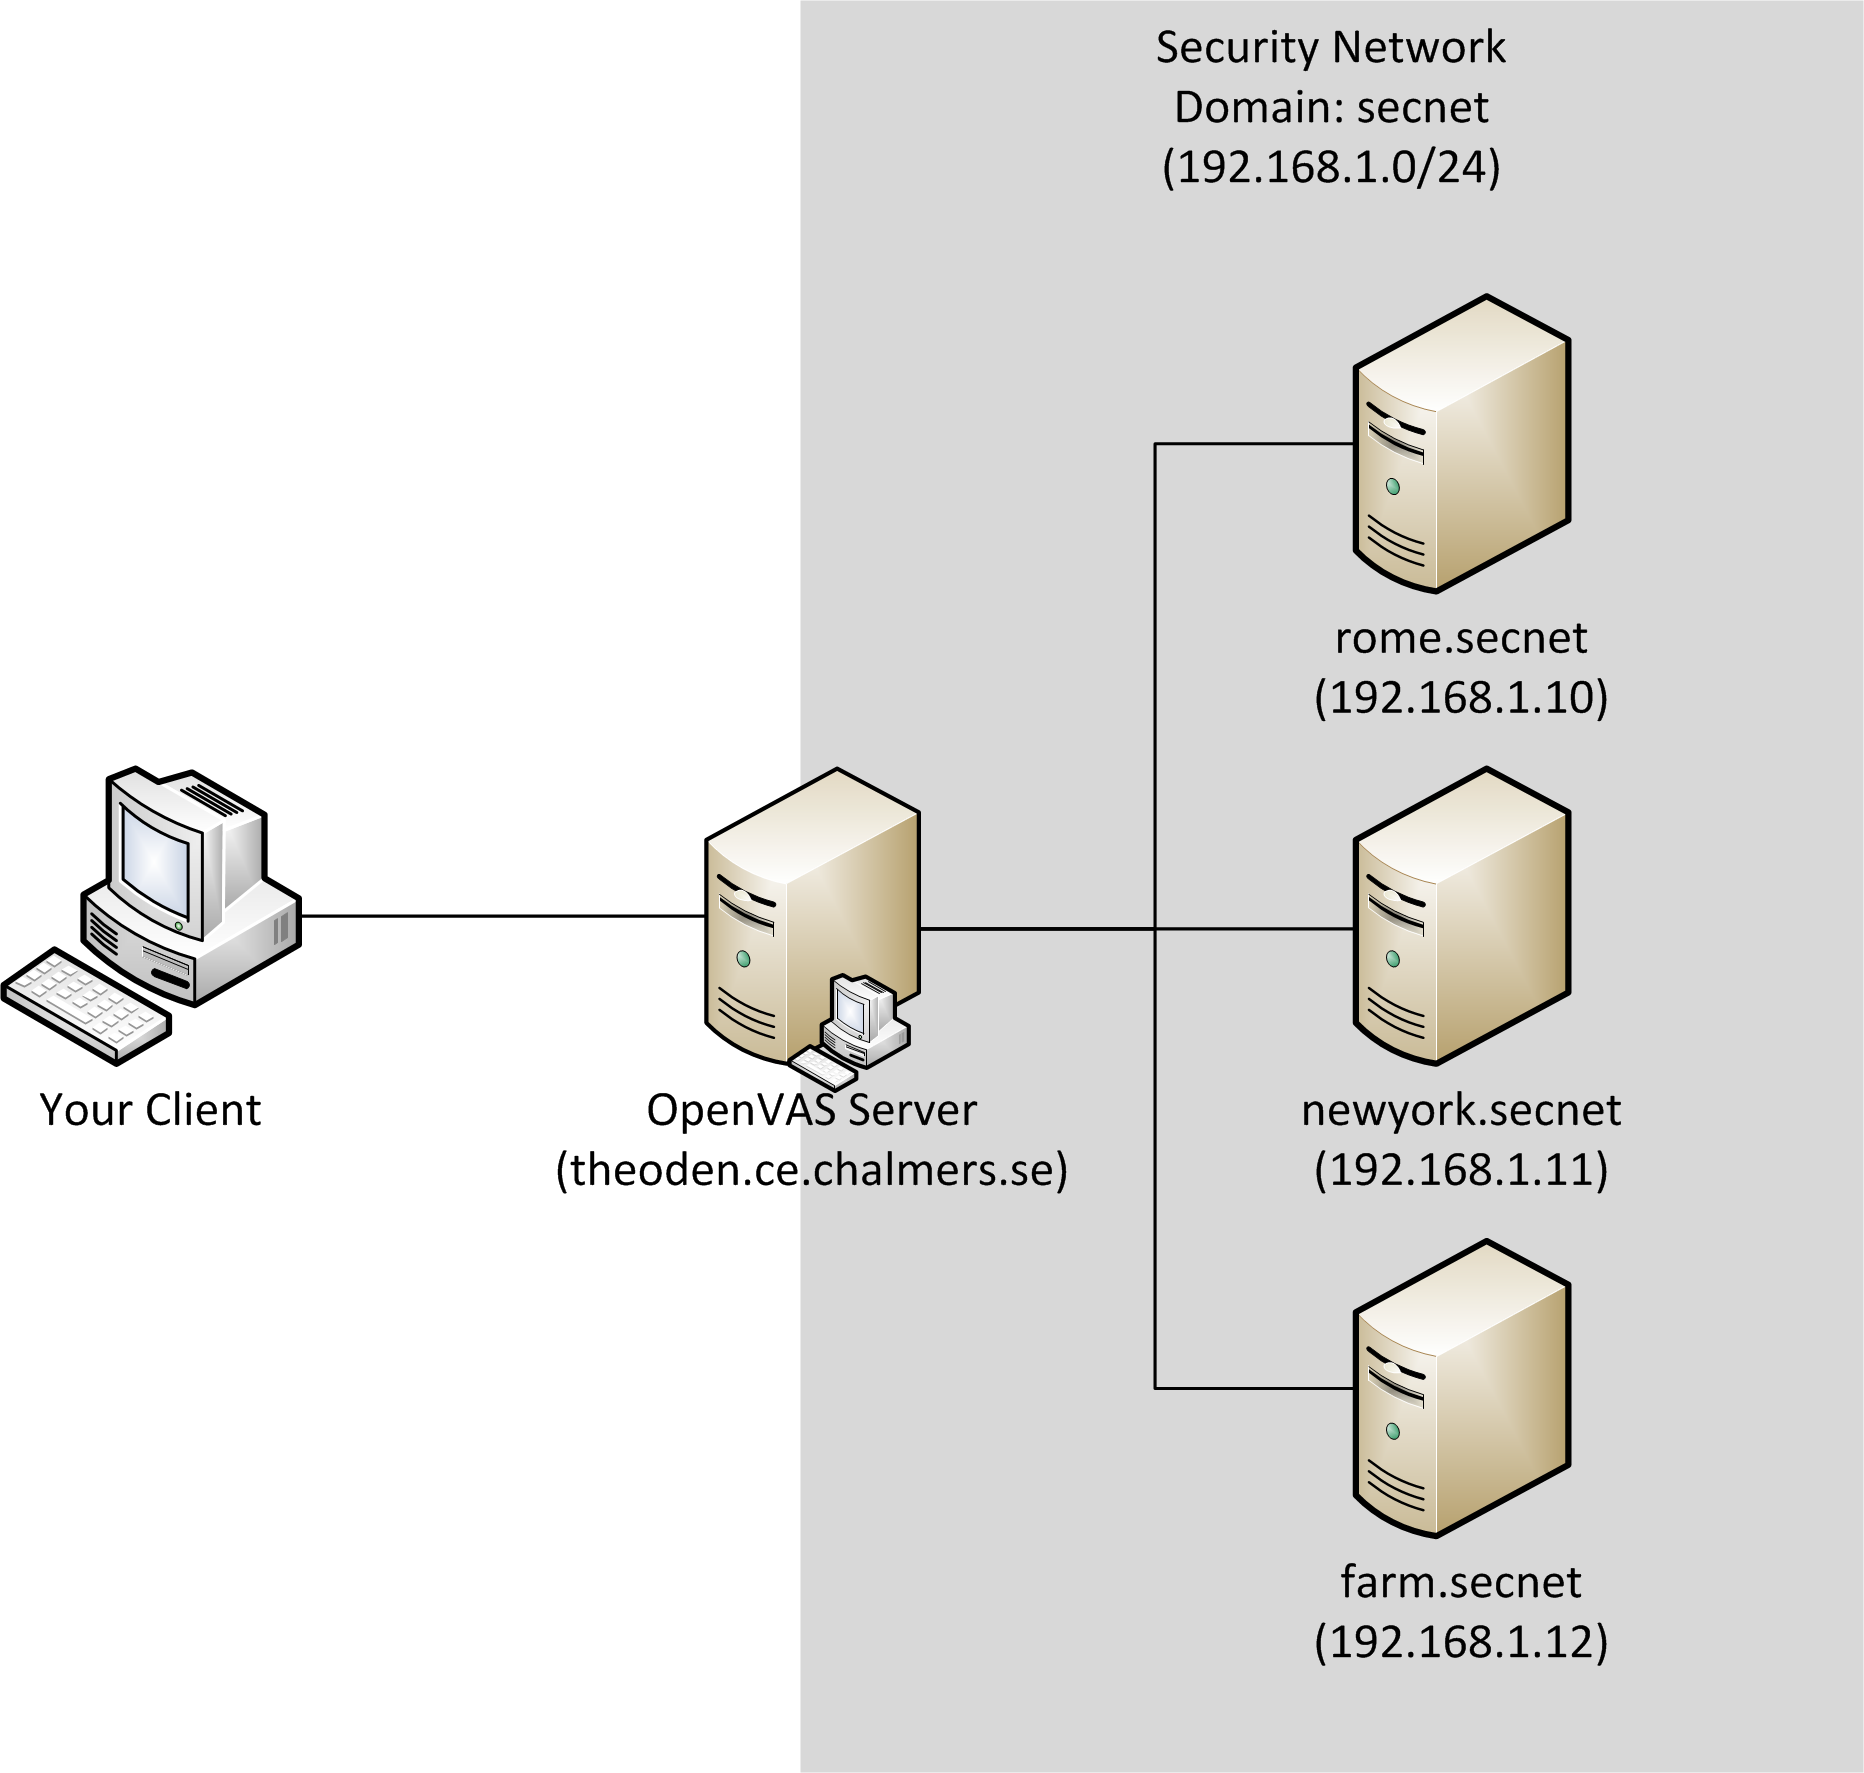
\includegraphics[scale=.4]{figures/setup.png}
  \caption{The network setup} \label{fig:setup}
\end{figure}



\subsection{Port Scanning}
\label{sub:port_set}

A set of tests in OpenVAS, called “Port Scanners”, were used to perform the port scanning, see Figure \ref{fig:portscanners}. \\

\noindent These NVTs where chosen so that a thorough port scan were conducted, and the open ports on the target will be displayed clearly. By doing this, information is gained on which ports on the target there are services listening for incoming connections. This is also similar to what a potential attacker would do.

\begin{figure}[htb]
  \centering
  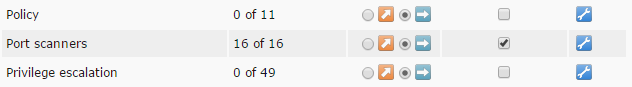
\includegraphics[scale=.4]{figures/port_nvt}
  \caption{Port Scanners NVT} \label{fig:portscanners}
\end{figure}

\newpage

\subsection{Service fingerprinting}
\label{sub:finger_set}
The settings we used in this section is the ones presented in Figures \ref{fig:general} and \ref{fig:service}

\begin{figure}[b!]
  \centering
  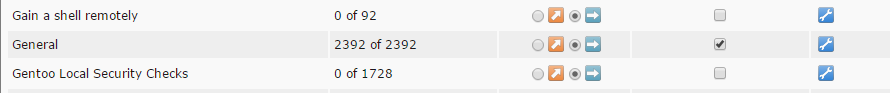
\includegraphics[scale=.4]{figures/general_nvt}
  \caption{General NVT} \label{fig:general}
\end{figure}

\begin{figure}[b!]
  \centering
  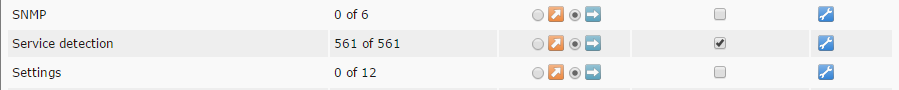
\includegraphics[scale=.4]{figures/service_nvt}
  \caption{Service detection NVT} \label{fig:service}
\end{figure}

\subsubsection{Service Fingerprinting}
To see which kind of services are running on the target system, OpenVAS was set up to try to get identifying information from them. Here the NVT families used were the ones collected in the NVT families “General” and “Service detection”. In addition to the self-explaining “Service detection”, “General” was added to broaden the detection possibilities.

\subsubsection{Remote Host Fingerprinting}
When doing this fingerprinting we will try to conclude what information is revealed of the system, in form of operative system such as Windows or Linux. 


\subsection{Vulnerability Scanning}
When the vulnerability scan was preformed, the predefined scan “full and fast” was used in order to detect all possible issues, see Figure \ref{fig:vulner}.

\begin{figure}[htb]
  \centering
  
\includegraphics[scale=.4]{figures/full_fast}
  \caption{Vulnerability scan} \label{fig:vulner}
\end{figure}


\section{Results}

As shown in Table \ref{tab:open_ports}, there are a number of open ports that belongs to relatively well known services. There is no imminent threat on these ports, although some services might be old and unused, it depends on what services on the host that are actually in use. \\

\noindent The services detected are presented in Table \ref{tab:service_fingerprint}, even though there are very few of them.


\subsection{Port Scanning}

When performing a port scan on the system, the ports found to be open are listed in Table \ref{tab:open_ports}. If the server is not part of a Microsoft Windows network, it should be considered to close the Windows related services and ports. Nothing abnormal was found. 

\begin{table}[htb]
 \centering
 \caption{Information about open ports} \label{tab:open_ports}
 \begin{tabular}{m{3cm}m{3cm}p{5cm}p{2cm}} \toprule
     \textbf{Port Number} & \textbf{Service Name} & 
     \textbf{Service Task} &  \textbf{Suggestion} \\ \midrule
        53      &   DNS         &   Domain Name System  &   Keep    \\
        80/8080 &   HTTP        &   Web traffic         &   Keep    \\
        143/993 &   IMAP/ \newline IMAPS  &   Email retrieval     &   Keep    \\
        445     &   Microsoft-DS & Microsoft network services \footnotemark[1] &   Keep\footnotemark[2]  \\ 
        139     &   NetBIOS Session Service &  Used by Microsoft-DS & Keep\footnotemark[2] \\
        110/995 &   POP3/ \newline POP3S  &   Email retrieval     &   Keep \\
        22      &   SSH  &   Secure data communication &   Keep \\
\bottomrule
 \end{tabular} 
\end{table}
\footnotetext[1]{Includes 'Active Directory: authentication and authorization' and 'SMB: File and printer sharing'}
\footnotetext[2]{Keep if the network rely on MS services related to this server}

\newpage

\subsection{Fingerprinting}


\subsubsection{Services}
\label{ssub:services_result}
As seen in Table \ref{tab:service_fingerprint}, one service was identified from the service fingerprinting scan, a Domain Name System (DNS) server called bind with the version number 9.7.0-p1. This version was released in 2010 and is outdated. \\

\noindent However, when performing the vulnerability scan, the fingerprints of the services listed in Table \ref{tab:vul_fingerprint} were found. \\

\noindent Of interest here is that all the listed services are old and outdated. Apache Tomcat 6.0.24 is a java servlet/web server that was released in 2010. Being published in 2009, the installed version of Apache HTTP web server is one year older than its java counterpart. The SMB server, Samba, is used for Linux/UNIX program interoperability with Windows and the current version dates back to 2010. Also OpenSSH, used for secure connections between computers, is of a version from 2010. All of the aforementioned services have multiple known security vulnerabilities.

\begin{table}[htb]
 \centering
 \caption{Service fingerprint} \label{tab:service_fingerprint}
 \begin{tabular}{m{4cm}p{3cm}} \toprule
 \textbf{Service} & \textbf{Version} \\ \midrule
 DNS server & bind 9.7.0-p1 \\ \bottomrule
 \end{tabular} 
\end{table}

\begin{table}[htb]
 \centering
 \caption{Vulnerability scan fingerprint} \label{tab:vul_fingerprint}
 \begin{tabular}{m{4cm}p{3cm}} \toprule
 \textbf{Service} & \textbf{Version} \\ \midrule
    Java servlet web server    &   Apache \newline Tomcat 6.0.24 \\
    HTTP \newline web server            &   Apache 2.2.14 \\
    mail server                 &   Dovecot \\
    SMB server               &   Samba 3.4.7 \\
    OpenSSH             &   OpenSSH 5.3p1 \\
 \\ \bottomrule
 \end{tabular} 
\end{table}


\subsubsection{Remote Host}

Analysing the information gained by the vulnerability scan, the system's operating system were confirmed to be of the Linux distribution Ubuntu. Combining this knowledge with the information provided in 3.2.1, it is also possible determine that the version of Ubuntu is of the 10.04 LTS \cite{ubuntu, newsletter}. It was also found that the system is part of a SMB/Windows workgroup with the name “WORKGROUP”.


\subsection{Vulnerability Scan}

As mentioned in \ref{ssub:services_result}, the vulnerability scan revealed the version of many of the system's services and that they are outdated. With outdated software it is common that there are publicly known vulnerabilities and weaknesses. OpenVAS classifies the threats found in the vulnerability scan by severity, high, medium and low. In the performed particular scan there were six high threats, ten medium threats and one low threat. \\

\noindent In Apache Tomcat 6.0.24, the java servlet/web server, the vulnerability scan found two high risk and five medium risk vulnerabilities. These security risks include, but are not limited to, that potential attackers can gain access to sensitive data and cause denial-of-service. \\

\noindent OpenSSL, in this case used for secure retrieval of email, were found to have two high risk and two medium risk vulnerabilities. The most critical vulnerability is the possibility of man-in-the-middle attacks; a session can be hijacked or compromised. \\

\noindent Remaining security risks classified as medium threats were a denial-of-service vulnerability in the SMB server Samba, risk of information-disclosure by the OpenSSH server and one vulnerability related to giving away timestamps, which can potentially open the system for denial-of-service attacks. \\

\noindent One threat were classified as low risk, the DNS server bind. The issues related to system's version of bind is mostly related to availability issues, as in cause the DNS server to crash or denial-of-service.

\section{Discussion} \label{sec:discussion}

\inlinetodo{Discuss your findings in different parts. Comment the information 
of Table~\ref{tab:recommendations} in the text. You may extend the table 
with more entries you found 
interesting. Make sure that the caption numbers are correct.
\newline
 \textbullet\  Elaborate on what needs to be done to improve the security.
\newline
 \textbullet\  Support your decisions with facts and recommendations from OpenVAS, such 
as severity of problem.
\newline
 \textbullet\  Compare your recommendations to the recommendations you made in 
Assignment 1.
}
\begin{table}[htb]
 \centering
 \caption{Summary of vulnerability scan recommendations} 
 \label{tab:recommendations}
 \begin{tabular}{m{2cm}p{4cm}p{7cm}} \toprule
 \textbf{Service Name} & \textbf{Problems} & \textbf{Suggestions} \\ \midrule
 & & \\
 & & \\
 & & \\
 & & \\
 & & \\ \bottomrule
 \end{tabular} 
\end{table}


\section{Conclusion} \label{sec:conclusion}

Our conclusion of this OpenVAS scan is that the host “Rome” is not secure, because of outdated software. The host could be considered secure if the software were to be updated. \\

\noindent Our first recommendation to secure the host is to implement a routine for software updates and patches. A designated person should be appointed to make sure that the software update routine is followed through, if there are more than one person that administrates the host. \\

\noindent Our second recommendation is to upgrade the operating system. From the vulnerability scan we can conclude that the OS installed on the host is the 'Ubuntu 10.04 LTS' system, which by now is quite old. To make sure that the OS is up to date, a system upgrade should be performed, some months after a new 'Long Time Support' OS is released from the vendor. 



\printbibliography
\addcontentsline{toc}{section}{References}

\appendix
\cleardoublepage
\section{Report from OpenVAS Vulnerability Scanning}
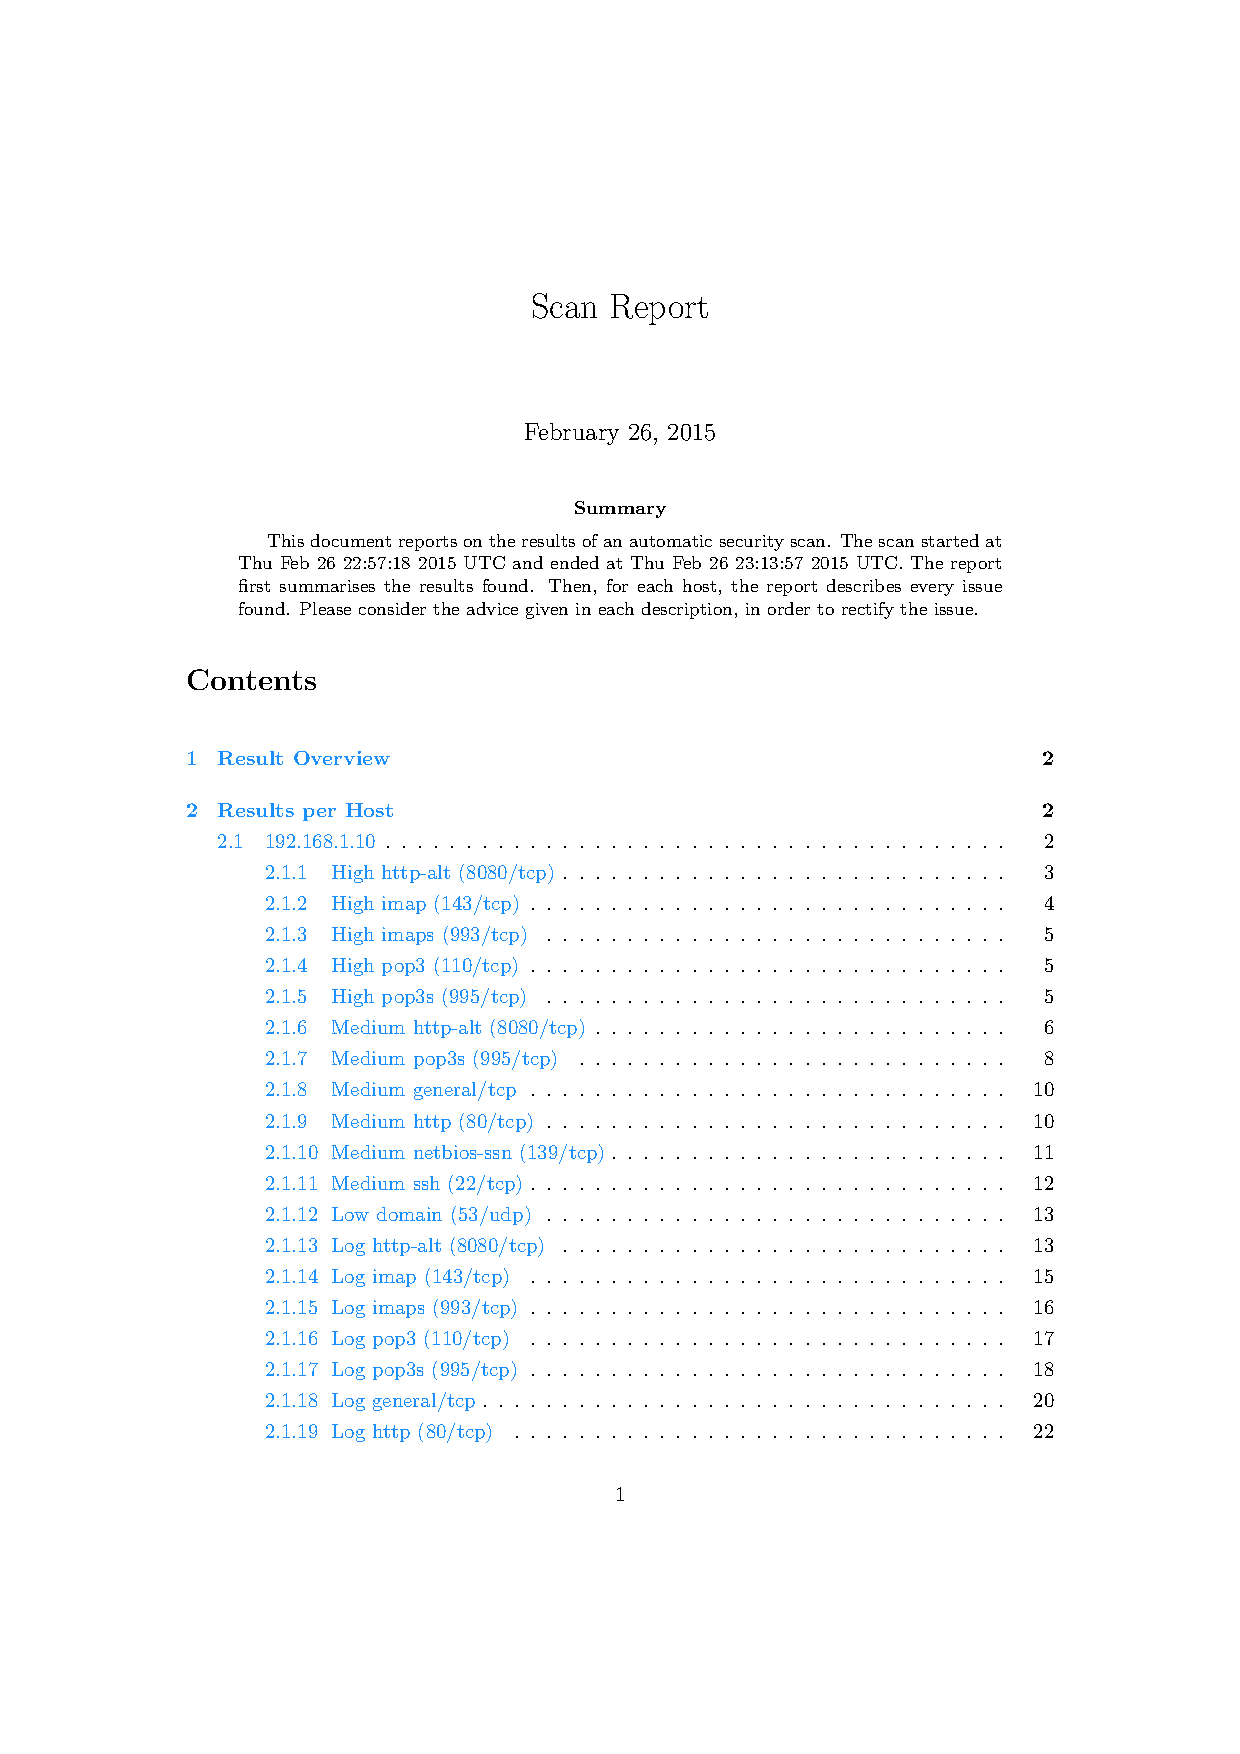
\includepdf[pages=-]{figures/report-full_scan.pdf}

\end{document}

